
\documentclass[review,3p,number,english]{elsarticle}
%\documentclass[letterpaper, 10 pt, conference]{ieeeconf}

%\IEEEoverridecommandlockouts
%\overrideIEEEmargins

%\usepackage{times}
%\usepackage{latexsym}
\usepackage{babel}
%\usepackage{algorithm}
%\usepackage{algorithmic}
%\usepackage[dvips]{graphicx}
\usepackage{amsthm}
\usepackage{amsmath}

\usepackage{mathrsfs}
%\usepackage[cmex10]{amsmath}
%\usepackage{amssymb}

\def\argmin{\mathop{\rm argmin}}
\def\argmax{\mathop{\rm argmax}}
\newcommand{\me}{\mathrm{e}}

\usepackage[final]{psfrag}
%\DeclareGraphicsExtensions{.eps,.ps,.PS,.EPS}

%---------------------------------------------------------
% DEFINICIONS R. VILANOVA
%
\def\q{z^{-1}}
\def\be{\begin{equation}}
\def\ee{\end{equation}}
\def\bea{\begin{eqnarray}}
\def\eea{\end{eqnarray}}

\def\conclusio#1{\vspace{0.5cm}
\centerline{\begin{tabular}{|p{4.75in}|}  \hline
\begin{center} {\em #1} \end{center}\\ \hline
\end{tabular} \vspace{0.5cm}}}

%
% NEW ENVIRONMENTS
%
% -----> Entorn Teorema (Theorem)
\newtheorem{Theorem}{Theorem}[section]

% -----> Entorn Lema (Lemma)
\newtheorem{Lemma}{Lemma}[section]

% -----> Entorn Corol.lari (Corollary)
\newtheorem{Corollary}{Corollary}[section]

% -----> Entorn Demostraci� (proof)
%\newenvironment{proof}{{\em Proof  : }}{\begin{flushright}
%$\Box$ \end{flushright}}

%
%---------------------------------------------------------
\journal{Journal of Process Control}

\begin{document}

\begin{frontmatter}

%\title{Improved PID Autotuning for balanced control operation}
\title{PID Autotuning for Weighted Servo/Regulation Control Operation}

\author[uab,ucr]{O. Arrieta}
\ead{Orlando.Arrieta@uab.cat,Orlando.Arrieta@ucr.ac.cr}

\author[ub]{A. Visioli}
\ead{antonio.visioli@ing.unibs.it}

\author[uab]{R. Vilanova}
\ead{Ramon.Vilanova@uab.cat}


\address[uab]{Departament de Telecomunicaci�\'o i d'Enginyeria de Sistemes, ETSE \\Universitat Aut\`onoma de Barcelona, 08193 Bellaterra, Barcelona, Spain}

\address[ucr]{Departamento de Autom\'atica, Escuela de Ingenier\'ia El\'ectrica \\Universidad de Costa Rica, San Jos\'e 11501-2060, Costa Rica}

\address[ub]{Dipartimento di Elettronica per l'Automazione, Facolt\`a di Ingegneria \\Universit\`a degli Studi di Brescia, Via Branze 38, 25213 Brescia, Italy}


%\maketitle

\begin{abstract}
This paper analyzes optimal controller settings for controllers
with One-Degree-of-Freedom (1-DoF)
Proportional-Integral-Derivative (PID) structure. A new analysis
is conducted from the point of view of the \emph{operating mode}
(either servo or regulation mode) of the control-loop and
\emph{tuning mode} of the controller. Performance of the optimal
tuning settings can be degraded when the operating mode is
different from that selected for tuning and obviously both
situations can be present in any control system. In this context,
a Weighted Performance Degradation index, that considers the
importance and balance between the servo and regulation operation
modes, is minimized and based on this minimization, an autotuning
procedure as a function of the normalized process dead-time is
proposed.
\end{abstract}

\begin{keyword}
PID Control \sep Performance Analysis \sep Automatic Tuning \sep
Genetic Algorithms
\end{keyword}

\end{frontmatter}

%-----------------------------------------
%
\section{Introduction}
%
%-------------------------------------------

Proportional-Integrative-Derivative (PID) {contro\-llers} are with
no doubt the most extensive option that can be found on industrial
control applications \cite{astromCEP2001}. Their success is mainly
due to its simple structure and to the physical meaning of the
corresponding three parameters (therefore making manual tuning
possible). This fact makes PID control easier to understand by the
control engineers than other most advanced control techniques. In
addition, the PID controller provides satisfactory performance in
a wide range of practical situations.

During the last years, in fact since the initial work of Ziegler
and Nichols \cite{zieglernichols42}, much work has been done
developing methods to determine the PID controller parameters (see
for example
\cite{astromJPC2004,skogestadJPC2003,kristianssonJPC2006}).
O'Dwyer \cite{odwyer2003} presents a collection of tuning rules
for PID controllers, which show their abundance.

Within the wide range of approaches to autotuning, optimal methods
have received special interest. These methods provide, given a
simple model process description -such as a
First-Order-Plus-Dead-Time (FOPDT) model- settings for optimal
closed-loop responses \cite{zhuangAthertonIEE1993}.

For One-Degree-of-Freedom (1-DoF) controllers, it is usual to
relate the tuning method to the expected operation mode for the
control system, known as \emph{servo} or \emph{regulation}.
Therefore, controller settings can be found for optimal set-point
or load-disturbance responses. This fact allows better performance
of the controller when the control system operates on the selected
tuned mode but, a degradation in the performance is expected when
the tuning and operation modes are different. Obviously there is
always the need to choose one of the two possible ways to tune the
controller, for set-point tracking or load-disturbances rejection.
In the case of 1-DoF PID, tuning can be optimal just for one of
the two operation modes. The main problem, about the Performance
Degradation analysis for both tuning modes, was previously
formulated in \cite{arrietaCSC2007} and some approaches related to
tuning methods and autotuning have been proposed in
\cite{arrietaMED2007,arrietaCDC2007}.

What is provided in this paper is a continuation of the these
ideas in order to find an \emph{intermediate} tuning for the
controller that improves the overall performance of the system,
considered as a \emph{trade-off} between servo and regulation
operation modes. The settings are determined from the combination
of the optimal ones for set-point and load-disturbance, presented
in \cite{zhuangAthertonIEE1993}, and taking into account the
balance between the importance of each one of the operation modes
for the control system (servo or regulation). The optimization is
here performed using genetic algorithms \citep{mitchell1998}.

The proposed new method considers a 1-DoF PID controller as an
alternative when an \emph{explicit} 2-DoF PID controller is not
available. It should be remembered that for the
Two-Degree-of-Freedom (2-DoF) PID controller, tuning is usually
optimal for regulation operation and suboptimal for servo-control,
where this suboptimal behavior is achieved using a set-point
weighting factor as an extra tuning parameter that gives the
second Degree-of-Freedom, to improve the tracking action. Also,
sometimes is not strictly necessary, or not justified, to increase
the number of the tuning parameters in contrast to the benefits
that could be obtained. It could be stated that the proposed
\emph{intermediate} tuning is a particular case that results in a
suboptimal tuning, when both operation modes may happen.

The paper is organized as follows. Next section introduces the
general problem formulation, with some related concepts. Section
\ref{methodology} presents the \emph{intermediate} tuning between
the parameters of both operation modes in such a way that a
Weighted Performance Degradation ($WPD$) is minimized; the results
are generalized in terms of an autotuning procedure that is
presented in Section \ref{autotuning}. Some examples are shown in
Section \ref{example} and the conclusions are drawn in Section
\ref{conclusions}.

%-----------------------------
%
\section{Problem Formulation}
%
%-----------------------------

\subsection{Control System Configuration}

We consider the unity-feedback system shown in Fig. \ref{1DOF},
where $P$ is the process and $K$ is the (1-DoF PID) controller.

\begin{figure}[h!]
    \begin{center}
        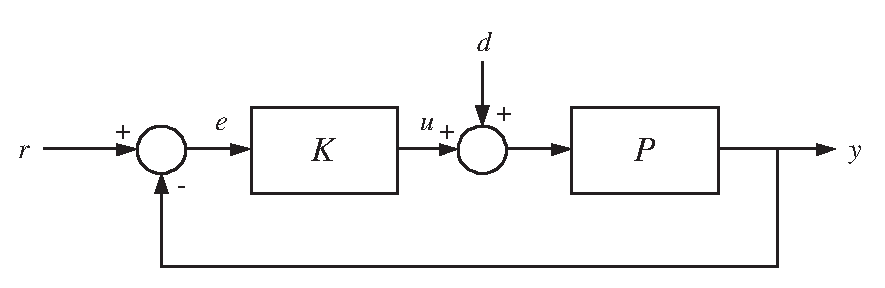
\includegraphics[width=0.6\linewidth]{1dof-3.eps}
        \caption{The considered feedback control system.}\label{1DOF}
    \end{center}
\end{figure}

The variables of interest can be described as follows:

\begin{itemize}

\item $y$ is the process output (controlled variable).

\item $u$ is the control signal.

\item $r$ is the set-point for the process output.

\item $d$ is the disturbance of the system.

\item $e$ is the control error $e=r-y$.

\end{itemize}

Also, the process $P$ is assumed to be modelled by a FOPDT
transfer function of the form

\be P(s) = \frac{K}{1+Ts}\me^{-Ls} \label{fopdt} \ee

\noindent where $K$ is the process gain, $T$ is the time constant
and $L$ is the dead-time. This model is commonly used in process
control because is simple and describes the dynamics of many
industrial processes approximately \cite{Astrombook06}.

The availability of FOPDT models in the process industry is a well
known fact. The generation of such model just needs for a very
simple step-test experiment to be applied to the process. This can
be considered as an advantage with respect to other methods that
need a more \emph{plant demanding} experiment such as methods
based on more complex models or even data-driven methods where a
sufficiently rich input needs to be applied to the plant. From
this point of view, to maintain the need for plant experimentation
to a minimum is a key point when considering industrial
application of a technique.

In this context, a common characterization of the process
parameters is done in terms of the normalized dead-time $\tau =
L/T$ \citep{visioli2006}. On the other hand, the ideal 1-DoF PID
controller with derivative time filter is considered

\be
K(s)=K_p\left (1+\frac{1}{T_i s}+\frac{T_d s}{1+(T_d/N)s} \right )
\label{pid} \ee

\noindent where $K_p$ is the proportional gain, $T_i$ is the
integral time constant and $T_d$ is the derivative time constant.
The derivative time noise filter constant $N$ usually takes values
within the range 5-33 \cite{Astrombook06,visioli2006}. Without
loss of generality, here we will consider $N=20$
\cite{zhuangAthertonIEE1993}.

\subsection{Servo and Regulation Operation Modes}

Considering the closed-loop system of Fig. \ref{1DOF} the process
output is given by

\be
y(s)=\frac{K(s)P(s)}{1+K(s)P(s)}r(s)+\frac{P(s)}{1+K(s)P(s)}d(s)
\label{processoutput} \ee

The process output $y$ depends of its two input signals, $r$ and
$d$ and from that, the system can operate in two different modes,
known as \emph{servo control} or \emph{regulatory control}. In the
first case, the control objective is to provide a good tracking of
the signal reference $r$, whereas in the second case is to
maintain the output variable at the desired value, despite
possible disturbances in $d$.

For the design of the control system, both operation modes must be
considered, however depending on the controller structure (e.g.
1-DoF PID), it is not always possible to specify different
performance behaviors for changes in the set-point and
load-disturbances.

For the servo operation mode, disturbances are not considered
($d(s)=0$), then (\ref{processoutput}) takes the form

\be
y_{sp}(s):=\frac{K(s)P(s)}{1+K(s)P(s)}r(s) \label{servooutput}\ee

For regulation operation mode, no changes in the set-point
reference are supposed (e.g. $r(s)=0$), then, process output would
be

\be y_{ld}(s):=\frac{P(s)}{1+K(s)P(s)}d(s)
\label{regoutput}\ee

\subsection{Set-Point and Load-Disturbance Tuning Modes}
\label{tuning-modes}

Controller tuning is one of the most important aspects in control
systems. For the selection of this, it is necessary to take into
account some aspects like: the controller structure, the
information that is available for the process and the
specifications that the output has to fulfill.

The analysis presented in this work is focused on the Integral
Square Error (ISE) criteria, $J=\int_0^{\infty} e(t)^2 dt$, which
is one of the most well known and most often used
\citep{Astrombook95}, however, the general analysis could be
developed in terms of any other performance criterion.

When the settings for optimal set-point (servo control) response
are considered, the controller parameters are adjusted according
to the following formulae \citep{zhuangAthertonIEE1993}

\bea K_p = \frac{a_1}{K} ( \tau )^{b_1},  & \qquad T_i =
\frac{T}{a_2+b_2 \tau}, &  \qquad T_d = a_3T (\tau )^{b_3}
\label{set_point_tuning_formulae} \eea

\noindent and for the optimal load-disturbance (regulatory
control) response

\bea K_p = \frac{a_1}{K} ( \tau )^{b_1},  & \qquad \frac{1}{T_i} =
\frac{a_2}{T}( \tau )^{b_2}, & \qquad T_d = a_3T (\tau )^{b_3}
\label{load_disturbance_tuning_formulae} \eea

\noindent where the corresponding values of $a_i$ and $b_i$ given
in Table \ref{optimal_settings}.

\begin{table}[htb!]
\begin{center}
\caption{Optimal PID Settings for Set-Point (SP) and
Load-Disturbance (LD)} \label{optimal_settings}
\begin{tabular}{c|cc|cc}
\hline \textbf{$\tau$ range} & \multicolumn{2}{c}{\textbf{0.1 -
1.0}} & \multicolumn{2}{c}{\textbf{1.1 - 2.0}} \\ \hline Tuning &
SP & LD & SP & LD \\
\hline
$a_1$ &  1.048 &  1.473 &  1.154 &  1.524 \\
$b_1$ & -0.897 & -0.970 & -0.567 & -0.735 \\
$a_2$ &  1.195 &  1.115 &  1.047 &  1.130 \\
$b_2$ & -0.368 & -0.753 & -0.220 & -0.641 \\
$a_3$ &  0.489 &  0.550 &  0.490 &  0.552 \\
$b_3$ &  0.888 &  0.948 &  0.708 &  0.851 \\
\hline
\end{tabular}
\end{center}
\end{table}

\subsection{Problem Statement}
\label{problem_formulation}

If the control-loop has always to operate on one of the two
possible operation modes (servo or regulator) the tuning choice
will be clear. However, when both situations occur, it may not be
so evident which are the most appropriate controller settings.

The analysis to answer the problem, presented previously as an
initial stage in \citep{arrietaCSC2007,arrietaMED2007},
concentrates on the Performance Degradation index which provides a
quantitative evaluation of the controller settings with respect to
the operation mode and the main objective is to reduce it.

Here, the question ``\emph{How to improve the performance when the
system operates also in a different mode that it was tuned for?}"
is treated by searching an \emph{intermediate} tuning for the
controller, between both optimal parameters settings for set-point
and load-disturbance, in order to reduce the global Weighted
Performance Degradation index.

Also, the selection of the servo/regulation \emph{trade-off}
tuning can be made to achieve a balanced performance behavior
between the operation modes.

\subsection{Motivation Example}
\label{motiv_ex}

In order to show the performance of the previously presented
settings and how this can degrade when the controller is not
operating according to the tuned mode, an example is provided.
This motivates the analysis to be presented in the next sections.

Consider the following plant transfer function, taken from
\cite{zhuangAthertonIEE1993}, and the corresponding FOPDT
approximation

\be P_1(s)=\frac{\me^{-0.5s}}{(s+1)^2} \approx
\frac{\me^{-0.99s}}{1+1.65s} \label{system_example} \ee

The application of the ISE tuning formulae for optimal set-point
response provides: $K^{sp}_p=1.657$, $T^{sp}_i=1.694$ and
$T^{sp}_d=0.513$, whereas the tuning for optimal load-disturbance
provides: $K^{ld}_p=2.418$, $T^{ld}_i=1.007$ and $T^{ld}_d=0.559$.

Fig. \ref{example1} shows the performance of both settings when
the control system is operating in both, servo and regulation
mode. It can be appreciated that the load-disturbance response of
the set-point tuning is closer to the optimal regulation one than
the load-disturbance tuning to the optimal servo tuning. Therefore
the observed Performance Degradation is larger for the
load-disturbance tuning. From a global point of view, it will seem
better to choose the set-point settings.

\begin{figure}[h!]
    \begin{center}
        \includegraphics[width=0.8\linewidth]{ex0.eps}
        \caption{Performance of the set-point (dotted) and load-disturbance (dashed)
        settings operating in both servo and regulation modes.}
        \label{example1}
    \end{center}
\end{figure}

%%-----------------------------------------
%
\section{Performance Degradation}
\label{performance-analysis}
%
%-------------------------------------------

The Performance Degradation concept for set-point and
load-disturbance tunings depending on the operation mode was
previously presented and developed in \cite{arrietaCSC2007} and it
is succinctly reproduced here for sake of completeness and because
it is important to have a clear idea of how is defined and
computed. There, the performance of the control system is measured
in terms of a performance index that takes into account the
possibility of an operation mode different from the selected one.
This motivates the redefinition of the ISE performance index as

\be J_x(z)=\int_0^{\infty} e(t,x,z)^2 dt
\label{generic_index_operating_mode} \ee

\noindent where $x$ denotes the \emph{operating mode} of the
control system and $z$ the selected operating mode for tuning,
i.e., the \emph{tuning mode}. Thus, we have $x \in
\left\{sp,ld\right\}$ and $z \in \left\{sp,ld\right\}$, where $sp$
states for set-point (servo) tuning and $ld$ for load-disturbance
(regulator) tuning. Obviously, for one specific process it has to
be verified that

\bea J_{sp}(sp) & \leq & J_{sp}(ld) \nonumber\\
J_{ld}(ld) & \leq & J_{ld}(sp) \nonumber \eea

Performance will not be optimal for both situations. The
Performance Degradation measure helps in the evaluation of the
loss of performance with respect to their optimal value.
Performance Degradation, $PD_x(z)$, will be associated to the
\emph{tuning mode} - $z$ -  and tested on the, opposite,
\emph{operating mode} - $x$ -. According to this, the Performance
Degradation of the load-disturbance tuning, $PD_{sp}(ld)$, will be
defined as

\be PD_{sp}(ld) = \left | \frac{J_{sp}(ld)
-J_{sp}(sp)}{J_{sp}(sp)} \right | \label{PD_load_disturbance} \ee

\noindent whereas the Performance Degradation associated to the
set-point tuning, $PD_{ld}(sp)$, will be

\be PD_{ld}(sp) = \left | \frac{J_{ld}(sp)
-J_{ld}(ld)}{J_{ld}(ld)} \right |. \label{PD_set_point} \ee

Note that, because the controller settings expressed through
(\ref{set_point_tuning_formulae}) and
(\ref{load_disturbance_tuning_formulae}) have explicit dependence
on the process normalized dead-time $\tau$, it is worth taking
into account that, for the PID application, the Performance
Degradation will also depend on $\tau$. Fig. \ref{PerfDegradation}
shows the performance analysis for the normalized dead-time ranges
where PID controller settings are provided by
\cite{zhuangAthertonIEE1993}.

\begin{figure}[h!]
    \begin{center}
        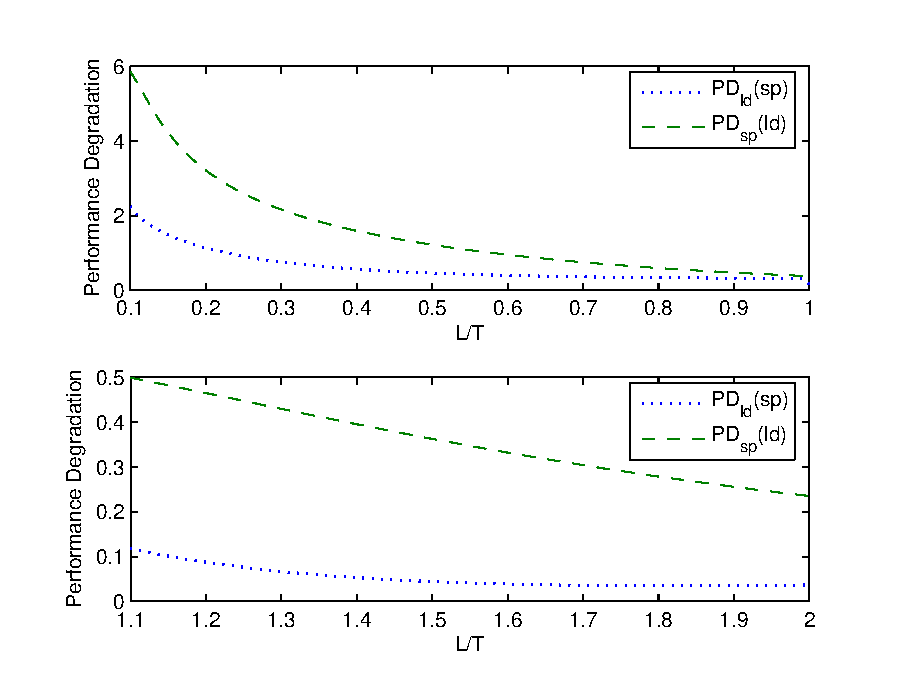
\includegraphics[width=0.8\linewidth]{PerfDeg.eps}
        \caption{Performance Degradation of set-point (sp) and load-disturbance (ld) tunings for ISE criteria with respect to the
        normalized dead-time $L/T$.}
        \label{PerfDegradation}
    \end{center}
\end{figure}

Note also that Performance Degradation is a decreasing function of
the normalized dead-time, taking very high values for processes
with small normalized dead-time.

The final decision for the choice of the appropriate tuning mode
will depend on the preference or importance that is given for the
system operation as regulator or as servo. However, if both
situations are likely to occur, Fig. \ref{PerfDegradation}
suggests a set-point based tuning is to be preferred, because it
provides lower Performance Degradation than load-disturbance
tuning.

%%-----------------------------------------------------------------------
%
\section{\emph{Intermediate} Tuning for Balanced Servo/Regulation Operation}
\label{methodology}
%
%-----------------------------------------------------------------------

The tuning approaches presented in subsection \ref{tuning-modes}
can be considered extremal situations. The controller settings are
obtained by considering exclusively one mode of operation. This
may generate, as it has been shown in the previous section, quite
poor performance if the non-considered situation happens. This
fact suggests to analyze if, by loosing some degree of optimality
with respect to the tuning mode, the Performance Degradation can
be reduced when the operation is different to the selected one for
tuning.

Based on this observation we suggest to look for an
\emph{intermediate} controller. In order to define this
exploration, we need to define the search-space and the overall
Performance Degradation index to be minimized. Obviously the
solution will depend on how this factors are defined.

The search of the controller settings that provide a
\emph{trade-off} performance for both operating modes could be
stated in terms of a completely new optimization procedure.
However, we would like to take advantage of the autotuning
formulae (like (\ref{set_point_tuning_formulae}) and
(\ref{load_disturbance_tuning_formulae})), in order to keep the
procedure, as well as the resulting controller expression, in
similar simple terms. Therefore, the resulting controller settings
could be considered as an extension of the optimal ones. On this
basis we define a controller settings family parameterized in
terms of a vector as

\be \overline{\gamma} = \left [\gamma_1,
\gamma_2, \gamma_3 \right] \ee

\noindent where $\gamma_i$ is a variable for each controller
parameter ($K_p$, $T_i$, $T_d$) that allows searching for the
\emph{intermediate} tuning. The values for this factor are
restricted to $\gamma_i \in [0,1]\quad i=1,2,3$. Also, the
set-point tuning will correspond to a contour constraint for each
$\gamma_i=0$, whereas the load-disturbance tuning corresponds to
$\gamma_i=1$. Fig. \ref{gamma} shows graphically the procedure and
the application for the 1-DoF PID controller tuning.

\begin{figure}[h!]
    \begin{center}
        %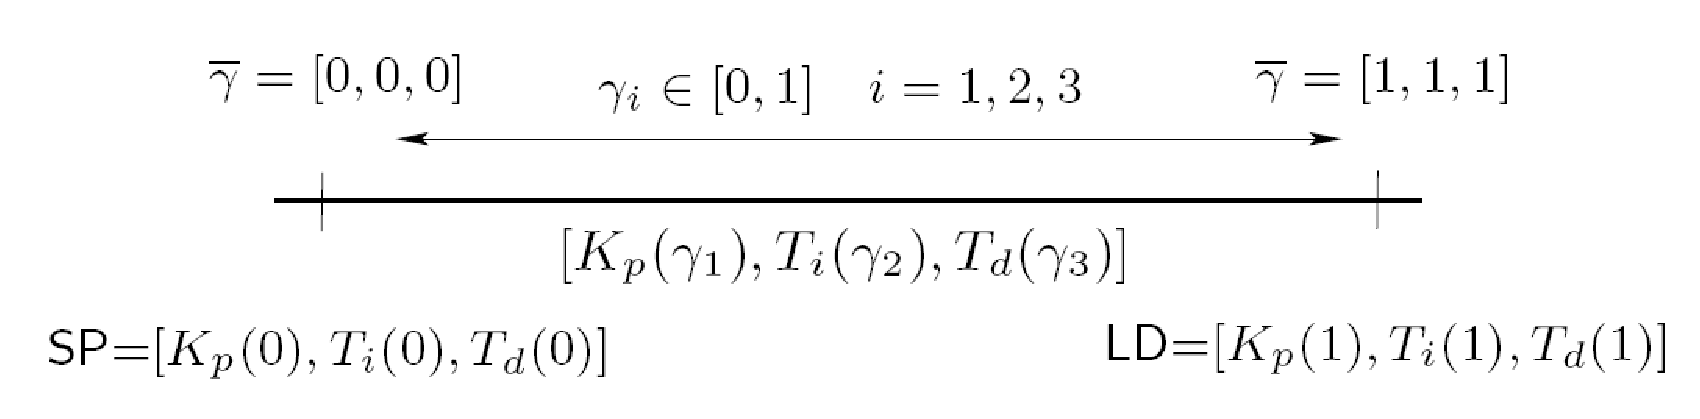
\includegraphics[scale=0.4]{gammaS.eps}
        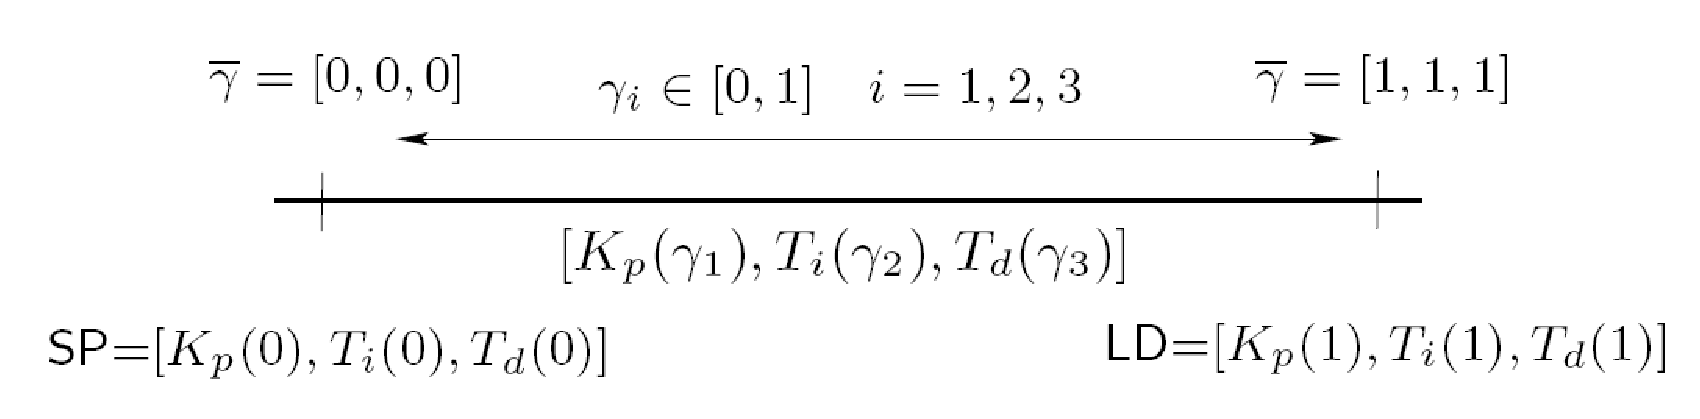
\includegraphics[width=0.8\linewidth]{gammaS.eps}
        \caption{$\overline{\gamma}-tuning$ procedure for the search of the \emph{intermediate} controller.}\label{gamma}
   \end{center}
\end{figure}

The controller settings family $[K_p(\gamma_1), T_i(\gamma_2),
T_d(\gamma_3)]$ will be generated by a linear evolution for the
parameters from the set-point tuning to the load-disturbance one
and the other way around. Therefore,
\bea
K_p(\gamma_1) & = & \gamma_1 K_p^{ld}+ (1-\gamma_1)K_p^{sp} \nonumber \\
T_i(\gamma_2) & = & \gamma_2 T_i^{ld}+ (1-\gamma_2)T_i^{sp} \label{gammaS_tuning_formulae}\\
T_d(\gamma_3) & = & \gamma_3 T_d^{ld}+ (1-\gamma_3)T_d^{sp}
\nonumber \eea

\noindent where $\gamma_i \in [0,1]\quad i=1,2,3$ and $[K_p^{sp},
T_i^{sp}, T_d^{sp}]$ and $[K_p^{ld}, T_i^{ld}, T_d^{ld}]$ stand
for the set-point and load-disturbance settings for $[K_p, T_i,
T_d]$ respectively.

Now, in order to define a global Performance Degradation
($\mathit{PD}$) index, the previously defined terms
(\ref{PD_load_disturbance}) and (\ref{PD_set_point}) need to be
extended. Note that the Performance Degradation was associated to
the \emph{tuning mode}, therefore tested against the opposite
\emph{operating mode}. Now, for every combination of
$\overline{\gamma}$ the Performance Degradation needs to be
measured with respect to both operating modes (because the
corresponding $\overline{\gamma}-tuning$ does not necessarily
corresponds to an operating mode). Hence,

\begin{itemize}
\item $PD_{sp}(\overline{\gamma})$ will represent the Performance
Degradation of the $\overline{\gamma}-tuning$ on servo operating
mode.

\be PD_{sp}(\overline{\gamma}) = \left |
\frac{J_{sp}(\overline{\gamma}) - J_{sp}(sp)}{J_{sp}(sp)} \right |
\label{PD_gamma_servo} \ee

\item $PD_{ld}(\overline{\gamma})$ will represent the Performance
Degradation of the $\overline{\gamma}-tuning$ on regulation
operating mode.

\be PD_{ld}(\overline{\gamma}) = \left |
\frac{J_{ld}(\overline{\gamma}) - J_{ld}(ld)}{J_{ld}(ld)} \right |
\label{PD_gamma_disturbance} \ee
\end{itemize}

From these Performance Degradation definitions, the overall
Performance Degradation is introduced and interpreted as a
function of $\overline{\gamma}$. There may be different ways to
define the $PD(\overline{\gamma})$ function, depending on the
importance associated to every operating mode (e.g. applying
weighting factors to each component). However, every definition
must satisfy the following contour constraints

\begin{displaymath}
PD(\overline{\gamma}) = \left \{ \begin{array}{ll} PD_{ld}(sp) &
\textrm{for  $\overline{\gamma}=\left[0,
0, 0 \right]$}\\
PD_{sp}(ld) & \textrm{for  $\overline{\gamma}=\left[1, 1, 1
\right]$}
\end{array} \right.
\end{displaymath}

The most simple definition would be

\be PD(\overline{\gamma}) =
PD_{ld}(\overline{\gamma}) + PD_{sp}(\overline{\gamma})
\label{global_pd} \ee

This expression represents a compromise, or a balance, between
both losses of performance.

As it has been mentioned before, the greatest loss of performance
occurs when the load-disturbance tuning operates as a servo mode.
Therefore, $PD_{sp}(\overline{\gamma})$ will be the largest
component of the global expression of $PD(\overline{\gamma})$ and
in the oppositive side $PD_{ld}(\overline{\gamma})$ the smallest
one. This causes that the percentage reduction of $\mathit{PD}$
that can be obtained from the $PD_{ld}$ side is lower than the one
for the $PD_{sp}$ part. A balanced reduction of
$PD(\overline{\gamma})$ from both Performance Degradations is
possible by introducing weighting factors associated to each
operating mode \cite{arrietaCSC2007}. This idea can be applied
rewriting (\ref{global_pd}) as

\be WPD(\overline{\gamma};\alpha) = \alpha
PD_{ld}(\overline{\gamma}) + (1-\alpha) PD_{sp}(\overline{\gamma})
\label{alpha_pd} \ee

\noindent that we call Weighted Performance Degradation
($\mathit{WPD}$) index, where $\alpha \in [0,1]$ is the weight
factor and indicates which of the two possible operation modes is
preferred or more important.

One way to express the importance between both operation modes,
could be the total time that the system operates in each one of
them. For example, a system that operates the 75\% of the time as
a regulator (or viceversa 25\% as a servo), $\alpha=0.75$.
However, the $\alpha$ parameter allows to make a more general
choice for the preference of the system operation (not only taking
into account the time for each operation mode).

Note also that (\ref{alpha_pd}) with $\alpha=0.50$, represents an
equivalent expression obtained previously in (\ref{global_pd})
that gives the same significance for both operation modes.

The \emph{intermediate} tuning will be determined by proper
selection of $\overline{\gamma} = \left [\gamma_1, \gamma_2,
\gamma_3 \right]$. This choice will correspond to the solution of
the following optimization problem,

\be \overline{\gamma}_{op} := \left [\gamma_{1op}, \gamma_{2op},
\gamma_{3op} \right ] = arg \left
[\min_{\overline{\gamma}}WPD(\overline{\gamma};\alpha) \right ]
\label{gamma_optimization}\ee

It is obvious that $\alpha=0$ means
\be WPD(\overline{\gamma};0) =
PD_{sp}(\overline{\gamma}) \label{alpha_pd0} \ee

\noindent and of course the $\overline{\gamma}_{op}$ that
minimizes the Performance Degradation for servo operation mode
(\ref{alpha_pd0}), is the one that corresponds to the set-point
tuning ($\overline{\gamma}=[0,0,0]$). On the other side,
$\alpha=1$ is equivalent to

\be WPD(\overline{\gamma};1) = PD_{ld}(\overline{\gamma})
\label{alpha_pd1} \ee

\noindent and the tuning that minimizes the Performance
Degradation for regulation operation (\ref{alpha_pd1}) is the
load-disturbance tuning that equals to
$\overline{\gamma}=[1,1,1]$.

The optimal values (\ref{gamma_optimization}) jointly with
(\ref{gammaS_tuning_formulae}), give a tuning formula that
provides a worse performance than the optimal settings operating
in the same way but also a lower degradation in the performance
when the \emph{operating mode} is different from the \emph{tuning
mode}.

%-----------------------------------------------------------------------
%
\section{\emph{Intermediate} Tuning for Balanced Servo/Regulation Operation}
\label{methodology}
%
%-----------------------------------------------------------------------

The tuning approaches presented in subsection \ref{tuning-modes}
can be considered extremal situations. The controller settings are
obtained by considering exclusively one mode of operation. This
may generate, as it has been shown in the previous section, quite
poor performance if the non-considered situation happens. This
fact suggests to analyze if, by loosing some degree of optimality
with respect to the tuning mode, the Performance Degradation can
be reduced when the operation is different to the selected one for
tuning.

Based on this observation we suggest to look for an
\emph{intermediate} controller. In order to define this
exploration, we need to define the search-space and the overall
Performance Degradation index to be minimized. Obviously the
solution will depend on how this factors are defined.

The search of the controller settings that provide a
\emph{trade-off} performance for both operating modes could be
stated in terms of a completely new optimization procedure.
However, we would like to take advantage of the autotuning
formulae (like (\ref{set_point_tuning_formulae}) and
(\ref{load_disturbance_tuning_formulae})), in order to keep the
procedure, as well as the resulting controller expression, in
similar simple terms. Therefore, the resulting controller settings
could be considered as an extension of the optimal ones. On this
basis we define a controller settings family parameterized in
terms of a vector as

\be \overline{\gamma} = \left [\gamma_1, \gamma_2, \gamma_3
\right] \ee

\noindent where $\gamma_i$ is a variable for each controller
parameter ($K_p$, $T_i$, $T_d$) that allows searching for the
\emph{intermediate} tuning. The values for this factor are
restricted to $\gamma_i \in [0,1]\quad i=1,2,3$. Also, the
set-point tuning will correspond to a contour constraint for each
$\gamma_i=0$, whereas the load-disturbance tuning corresponds to
$\gamma_i=1$. Fig. \ref{gamma} shows graphically the procedure and
the application for the 1-DoF PID controller tuning.

\begin{figure}[h!]
    \begin{center}
        %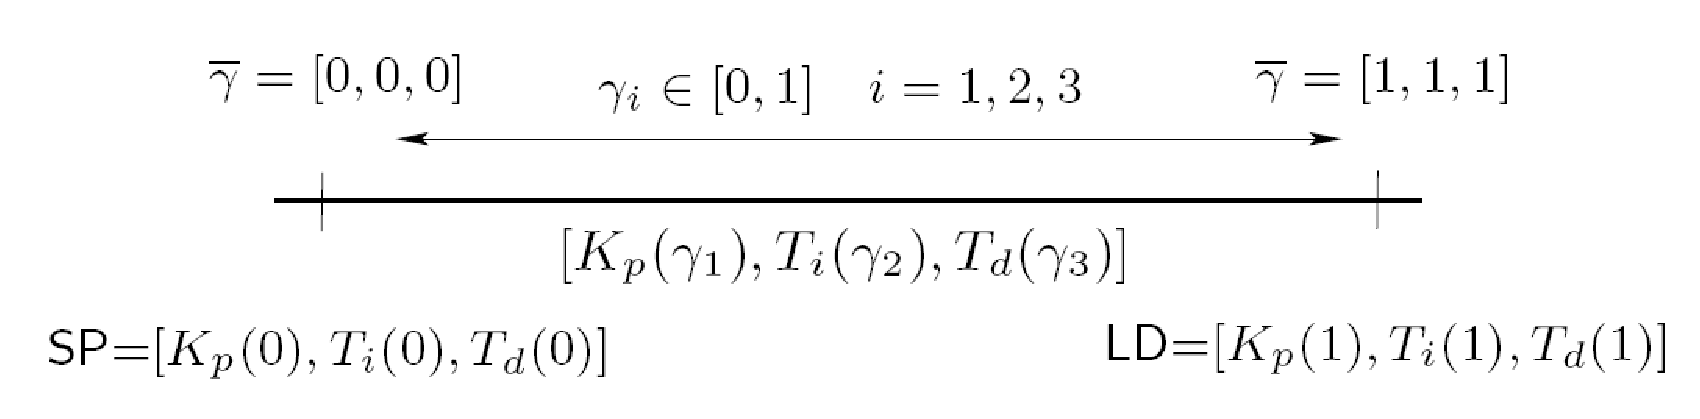
\includegraphics[scale=0.4]{gammaS.eps}
        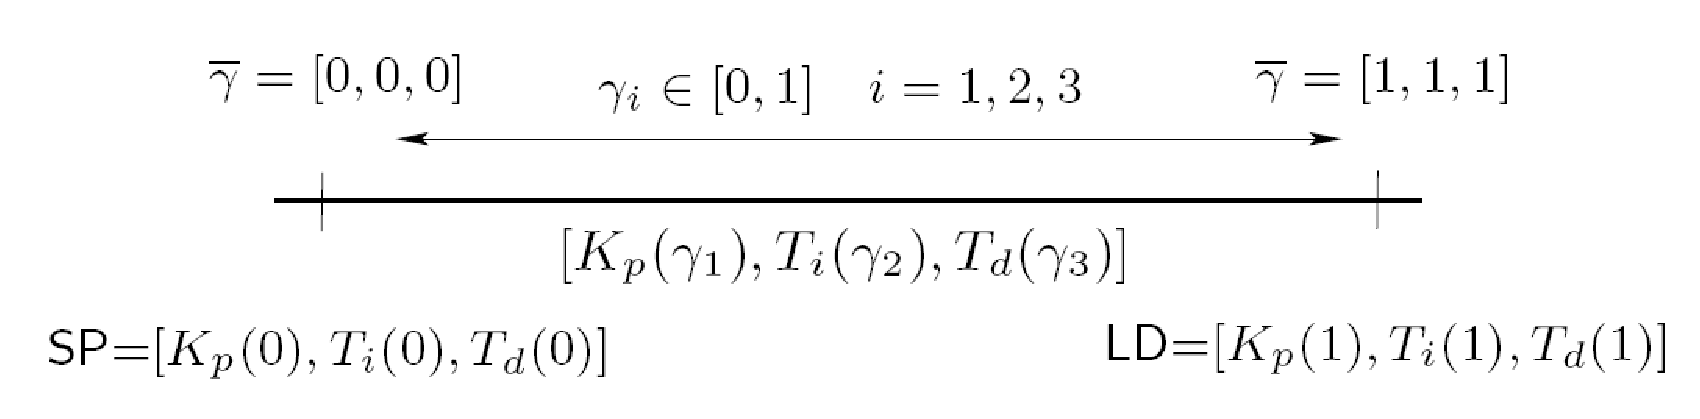
\includegraphics[width=0.8\linewidth]{gammaS.eps}
        \caption{$\overline{\gamma}-tuning$ procedure for the search of the \emph{intermediate} controller.}\label{gamma}
   \end{center}
\end{figure}

The controller settings family $[K_p(\gamma_1), T_i(\gamma_2),
T_d(\gamma_3)]$ will be generated by a linear evolution for the
parameters from the set-point tuning to the load-disturbance one
and the other way around. Therefore, \bea
K_p(\gamma_1) & = & \gamma_1 K_p^{ld}+ (1-\gamma_1)K_p^{sp} \nonumber \\
T_i(\gamma_2) & = & \gamma_2 T_i^{ld}+ (1-\gamma_2)T_i^{sp} \label{gammaS_tuning_formulae}\\
T_d(\gamma_3) & = & \gamma_3 T_d^{ld}+ (1-\gamma_3)T_d^{sp}
\nonumber \eea

\noindent where $\gamma_i \in [0,1]\quad i=1,2,3$ and $[K_p^{sp},
T_i^{sp}, T_d^{sp}]$ and $[K_p^{ld}, T_i^{ld}, T_d^{ld}]$ stand
for the set-point and load-disturbance settings for $[K_p, T_i,
T_d]$ respectively.

The Performance Degradation concept for set-point and
load-disturbance tunings depending on the operation mode was
previously presented and developed in \cite{arrietaCSC2007}.

There, the performance of the control system is measured in terms
of a performance index that takes into account the possibility of
an operation mode different from the selected one. This motivates
the redefinition of the ISE performance index as

\be J_x(z)=\int_0^{\infty} e(t,x,z)^2 dt
\label{generic_index_operating_mode} \ee

\noindent where $x$ denotes the \emph{operating mode} of the
control system and $z$ the selected operating mode for tuning,
i.e., the \emph{tuning mode}. Thus, we have $x \in
\left\{sp,ld\right\}$ and $z \in \left\{sp,ld\right\}$, where $sp$
states for set-point (servo) tuning and $ld$ for load-disturbance
(regulator) tuning.

Performance will not be optimal for both situations. The
Performance Degradation measure helps in the evaluation of the
loss of performance with respect to their optimal value.
Performance Degradation, $PD_x(z)$, will be associated to the
\emph{tuning mode} - $z$ -  and tested on the, opposite,
\emph{operating mode} - $x$ -. Now, for every combination of
$\overline{\gamma}$ the Performance Degradation needs to be
measured with respect to both operating modes (because the
corresponding $\overline{\gamma}-tuning$ does not necessarily
corresponds to an operating mode). Hence,

\begin{itemize}
\item $PD_{sp}(\overline{\gamma})$ will represent the Performance
Degradation of the $\overline{\gamma}-tuning$ on servo operating
mode.

\be PD_{sp}(\overline{\gamma}) = \left |
\frac{J_{sp}(\overline{\gamma}) - J_{sp}(sp)}{J_{sp}(sp)} \right |
\label{PD_gamma_servo} \ee

\item $PD_{ld}(\overline{\gamma})$ will represent the Performance
Degradation of the $\overline{\gamma}-tuning$ on regulation
operating mode.

\be PD_{ld}(\overline{\gamma}) = \left |
\frac{J_{ld}(\overline{\gamma}) - J_{ld}(ld)}{J_{ld}(ld)} \right |
\label{PD_gamma_disturbance} \ee
\end{itemize}

Note that, because the controller settings expressed through
(\ref{set_point_tuning_formulae}) and
(\ref{load_disturbance_tuning_formulae}) have explicit dependence
on the process normalized dead-time $\tau$, it is worth taking
into account that, for the PID application, the Performance
Degradation will also depend on $\tau$. Fig. \ref{PerfDegradation}
shows the performance analysis for the normalized dead-time ranges
where PID controller settings (set-point and load-disturbance),
are provided by \cite{zhuangAthertonIEE1993}.

\begin{figure}[h!]
    \begin{center}
        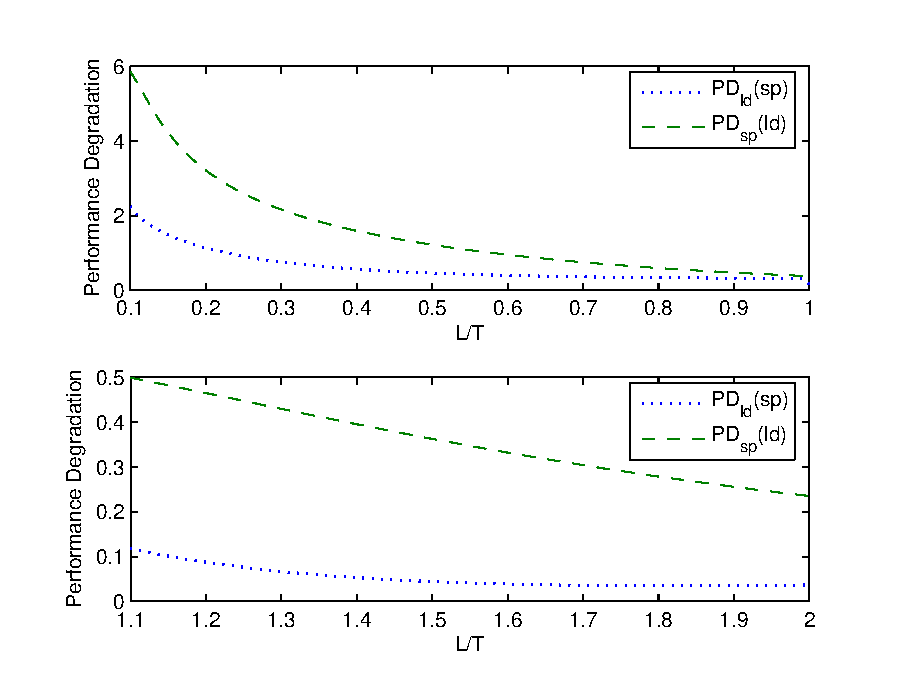
\includegraphics[width=0.8\linewidth]{PerfDeg.eps}
        \caption{Performance Degradation of set-point (sp) and load-disturbance (ld) tunings for ISE criteria with respect to the
        normalized dead-time $L/T$.}
        \label{PerfDegradation}
    \end{center}
\end{figure}

From the above Performance Degradation definitions, the overall
Performance Degradation is introduced and interpreted as a
function of $\overline{\gamma}$. There may be different ways to
define the $PD(\overline{\gamma})$ function, depending on the
importance associated to every operating mode (e.g. applying
weighting factors to each component). However, every definition
must satisfy the following contour constraints

\begin{displaymath}
PD(\overline{\gamma}) = \left \{ \begin{array}{ll} PD_{ld}(sp) &
\textrm{for  $\overline{\gamma}=\left[0,
0, 0 \right]$}\\
PD_{sp}(ld) & \textrm{for  $\overline{\gamma}=\left[1, 1, 1
\right]$}
\end{array} \right.
\end{displaymath}

The most simple definition would be

\be PD(\overline{\gamma}) = PD_{ld}(\overline{\gamma}) +
PD_{sp}(\overline{\gamma}) \label{global_pd} \ee

This expression represents a compromise, or a balance, between
both losses of performance.

As it has been mentioned before, the greatest loss of performance
occurs when the load-disturbance tuning operates as a servo mode.
Therefore, $PD_{sp}(\overline{\gamma})$ will be the largest
component of the global expression of $PD(\overline{\gamma})$ and
in the oppositive side $PD_{ld}(\overline{\gamma})$ the smallest
one. This causes that the percentage reduction of $\mathit{PD}$
that can be obtained from the $PD_{ld}$ side is lower than the one
for the $PD_{sp}$ part. A balanced reduction of
$PD(\overline{\gamma})$ from both Performance Degradations is
possible by introducing weighting factors associated to each
operating mode \cite{arrietaCSC2007}. This idea can be applied
rewriting (\ref{global_pd}) as

\be WPD(\overline{\gamma};\alpha) = \alpha
PD_{ld}(\overline{\gamma}) + (1-\alpha) PD_{sp}(\overline{\gamma})
\label{alpha_pd} \ee

\noindent that we call Weighted Performance Degradation
($\mathit{WPD}$) index, where $\alpha \in [0,1]$ is the weight
factor and indicates which of the two possible operation modes is
preferred or more important.

One way to express the importance between both operation modes,
could be the total time that the system operates in each one of
them. For example, a system that operates the 75\% of the time as
a regulator (or viceversa 25\% as a servo), $\alpha=0.75$.
However, the $\alpha$ parameter allows to make a more general
choice for the preference of the system operation (not only taking
into account the time for each operation mode).

Note also that (\ref{alpha_pd}) with $\alpha=0.50$, represents an
equivalent expression obtained previously in (\ref{global_pd})
that gives the same significance for both operation modes.

The \emph{intermediate} tuning will be determined by proper
selection of $\overline{\gamma} = \left [\gamma_1, \gamma_2,
\gamma_3 \right]$. This choice will correspond to the solution of
the following optimization problem,

\be \overline{\gamma}_{op} := \left [\gamma_{1op}, \gamma_{2op},
\gamma_{3op} \right ] = arg \left
[\min_{\overline{\gamma}}WPD(\overline{\gamma};\alpha) \right ]
\label{gamma_optimization}\ee

It is obvious that $\alpha=0$ means \be WPD(\overline{\gamma};0) =
PD_{sp}(\overline{\gamma}) \label{alpha_pd0} \ee

\noindent and of course the $\overline{\gamma}_{op}$ that
minimizes the Performance Degradation for servo operation mode
(\ref{alpha_pd0}), is the one that corresponds to the set-point
tuning ($\overline{\gamma}=[0,0,0]$). On the other side,
$\alpha=1$ is equivalent to

\be WPD(\overline{\gamma};1) = PD_{ld}(\overline{\gamma})
\label{alpha_pd1} \ee

\noindent and the tuning that minimizes the Performance
Degradation for regulation operation (\ref{alpha_pd1}) is the
load-disturbance tuning that equals to
$\overline{\gamma}=[1,1,1]$.

The optimal values (\ref{gamma_optimization}) jointly with
(\ref{gammaS_tuning_formulae}), give a tuning formula that
provides a worse performance than the optimal settings operating
in the same way but also a lower degradation in the performance
when the \emph{operating mode} is different from the \emph{tuning
mode}.

\emph{Remark:} It is important to note that the presented
procedure has just considered the performance with respect to the
proposed Performance Degradation index. Other closed-loop
characteristics such as stability robustness, tolerance to
parameter variation, etc. are not taken into account. How to
consider additional closed-loop characteristics is a subject of
current research. However it is clear that in order to include
such characteristics into consideration, they need to be part of
the original extreme tunings.

%-----------------------------------------------------------------------
%
\section{Optimization and Autotuning Rules}
\label{autotuning}
%
%-----------------------------------------------------------------------

To provide the possibility to specify any possible combination
between both operation modes, the index (\ref{alpha_pd}), with an
appropriated weight factor $\alpha$ and subjected to the
optimization (\ref{gamma_optimization}), gives the suitable
$\gamma_i$ values that provide the PID tuning according to
(\ref{gammaS_tuning_formulae}).

However, from a more practical point of view is unusual and very
difficult to say for example, that the regulation mode, in a
control system, has the 63\% of the importance (that means the
37\% for the servo). With this respect, we can establish a
categorization in order to make the analysis simpler and also to
help the choice of the weight factor. Therefore, depending on the
operation for the control system, we can identify the following
general cases:

\begin{itemize}

\item Operation only as a servo that means $\alpha=0$.

\item Operation only as a regulator that means $\alpha=1$.

\item Same importance for both system operation modes, servo and
regulation, that is equivalent to $\alpha=0.50$.

\item More importance for the servo than the regulation operation,
that can be expressed by $\alpha=0.25$.

\item More importance for regulator than servo, that can be
indicated as $\alpha=0.75$.

\end{itemize}

This broad classification allows for a qualitative specification
of the control system operation.

Here, the optimization was performed using genetic algorithms
\citep{mitchell1998}, taking problem (\ref{gamma_optimization}) as
the \emph{fitness function}. The implementation was using MATLAB
7.6.0(R2008a)\textregistered{ } for a \emph{population size} of 20
and a maximum number of \emph{generations} of 50.

The optimal solution was found for $\alpha=\{0.25, 0.50, 0.75\}$.
As we said before for $\alpha=\{0, 1\}$, as extreme situations,
the optimal tunings are the related to set-point and
load-disturbance presented previously in Subsection
\ref{tuning-modes}.

It is worth to say that at first the optimization was performed by
considering an enlarged search space for the $\overline{\gamma}$
vector, however, for the rare cases in which the optimal
$\gamma_i$ parameters were outside the interval $[0,1]$, the value
of the objective function was practically the same and, therefore,
it is preferred to constraint the search space in order to provide
a bounded controller's family that is easier to understand as are
presented of an \emph{intermediate} controller.

Tuning relations (\ref{gammaS_tuning_formulae}) allow to select
$\gamma_i$ values on the basis of \emph{trade-off} performance for
both operating modes. However, it would be desirable an automatic
methodology to choose this set of parameters without the need to
run the whole Weighted Performance Degradation analysis.

In order to pursue the previous idea, by repeating the problem
optimization posed in (\ref{gamma_optimization}) for the three
weighting factor and different values of the normalized dead-time
$\tau$, we can find an optimal set for each $\gamma_i$ parameter.
For each one of these groups, it is possible to approximate a
function to determine a general procedure that allows to find the
suitable values for the $\gamma_i$'s, that provide the best
\emph{intermediate} tuning. Results are adjusted to the general
expression as

\be
\gamma_i(\tau)=a+b\tau+c\tau^2 \qquad \tau \in [0.1,1.0] \cup
[1.1,2.0] \label{gammas-eq} \ee

\noindent where $a$, $b$ and $c$ are given in Table
\ref{gammas_settings}, according to the weighting factor $\alpha$
and for each $\gamma_i$ and $\tau$ range. Fig. \ref{gamma1fnc}
shows the followed procedure for $\alpha=0.50$ and the $\gamma_1$
case.

\begin{table}[htb!]
\begin{center}
\caption{$\overline{\gamma}_{\alpha}$ Settings for Autotuning}
\label{gammas_settings}
\begin{tabular}{cc|ccc|ccc}
\cline{2-8} & \textbf{$\tau$ range} &
\multicolumn{3}{c|}{\textbf{0.1 - 1.0}} &
\multicolumn{3}{c}{\textbf{1.1 - 2.0}} \\ \cline{2-8} & constant &
a & b & c & a & b & c \\ \hline
              & \multicolumn{1}{c|}{$\gamma_1$} &0.082 & 0.074 &0.138 &0.021 & 0.040 &-0.006 \\
$\alpha=0.25$ & \multicolumn{1}{c|}{$\gamma_2$} &0.896 &-1.238 &0.854 &0.097 &-0.723 & 0.173 \\
              & \multicolumn{1}{c|}{$\gamma_3$} &0.332 &-0.592 &0.508 &0.323 &-0.183 & 0.033 \\
\hline
              & \multicolumn{1}{c|}{$\gamma_1$} &0.093 & 0.547 &-0.106 & 1.162 &-1.258 & 0.406 \\
$\alpha=0.50$ & \multicolumn{1}{c|}{$\gamma_2$} &0.920 &-0.540 & 0.206 & 2.222 &-2.184 & 0.639 \\
              & \multicolumn{1}{c|}{$\gamma_3$} &0.831 &-1.197 & 0.548 &-0.436 & 0.941 &-0.334 \\
\hline
              & \multicolumn{1}{c|}{$\gamma_1$} &0.108 & 0.566 & 0.067 & 2.197 &-2.529 & 0.774 \\
$\alpha=0.75$ & \multicolumn{1}{c|}{$\gamma_2$} &0.869 &-0.271 & 0.129 & 1.312 &-1.021 & 0.296 \\
              & \multicolumn{1}{c|}{$\gamma_3$} &0.211 & 0.701 &-0.683 &-0.987 & 1.791 &-0.579 \\
\hline
\end{tabular}
\end{center}
\end{table}

\begin{figure}[htb!]
    \begin{center}
        %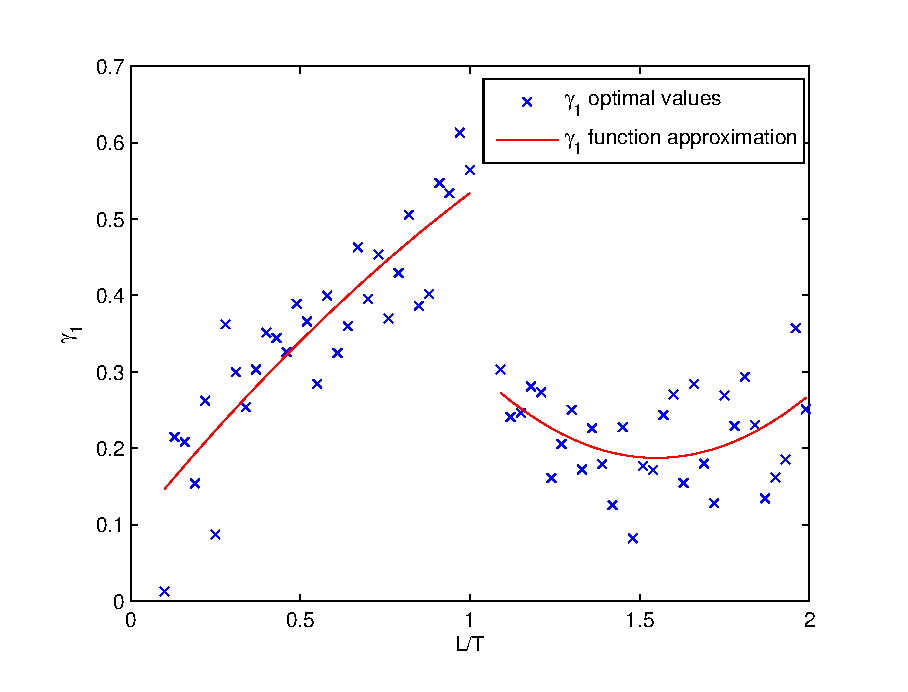
\includegraphics[scale=0.8]{gamma1function.eps}
        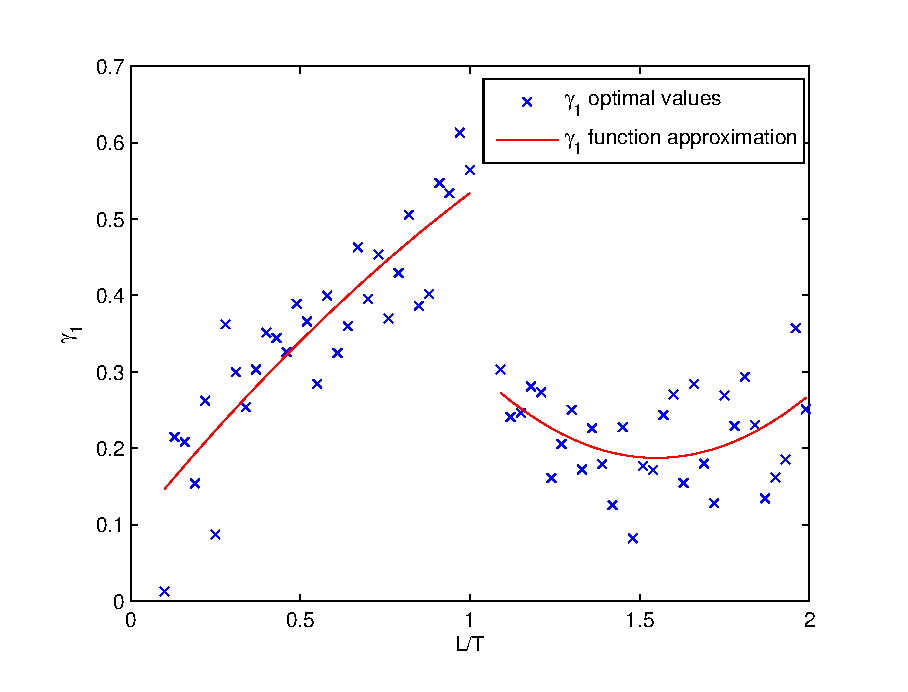
\includegraphics[width=0.8\linewidth]{gamma1function.eps}
        \caption{Optimal set for $\gamma_1$ parameter and the corresponding approximated function for $\alpha=0.50$}
        \label{gamma1fnc}
    \end{center}
\end{figure}

Equation (\ref{gammas-eq}) for each $\gamma_i$ along with the
settings (\ref{gammaS_tuning_formulae}) provide what we call here
$\overline{\gamma}_{\alpha}-autotuning$ for weighted
servo/regulation operation, that is the main contribution of this
paper.

%-----------------------------------------------------------------------
%
\section{Examples}
\label{example}
%
%-----------------------------------------------------------------------

This section presents several examples to illustrate how the
implementation of the $\overline{\gamma}_{\alpha}-autotuning$
improves the performance of the closed-loop system respect to the
both operation modes.

In all the examples it is supposed that the process output can
vary in the 0 to 100\% normalized range and that in the normal
operation point, the controlled variable has a value close to
70\%.

\subsection{Example 1}

Let us to consider the system (\ref{system_example}), shown before
as a \emph{Motivation Example}.

Table \ref{PID_parameters} shows the PID controller parameters for
the system (\ref{system_example}) using the
\cite{zhuangAthertonIEE1993} method and the proposed
$\overline{\gamma}_{\alpha}-autotuning$ with $\alpha=\{0.25, 0.50,
0.75\}$. Moreover, the corresponding system outputs responses to a
20\% set-point change followed by a -20\% load-disturbance change,
are shown in Fig. \ref{y_out} for the following tuning methods:
set-point, load-disturbance and
$\overline{\gamma}_{\alpha}-autotuning$ with its three possible
scenarios. The control signal is not shown for the sake of
brevity, however it can be easily guessed that it would be
smoother when the value of $\alpha$ is lower (see Example 3).

\begin{table}[h!]
\begin{center}
\caption{Example 1 - PID Controller Parameters}
\begin{tabular}{c|ccc}
\hline \textbf{tuning}               &$K_p$ &$T_i$ &$T_d$\\ \hline
$set-point(sp)$                               &1.657  &1.694  &0.513 \\
$load-disturbance(ld)$                        &2.418  &1.007  &0.559 \\
\hline
$\overline{\gamma}_{\alpha=0.25}-autotuning$  &1.791  &1.378  &0.520 \\
$\overline{\gamma}_{\alpha=0.50}-autotuning$  &1.949  &1.234  &0.527 \\
$\overline{\gamma}_{\alpha=0.75}-autotuning$  &2.016  &1.177  &0.531 \\
\hline
\end{tabular}
\label{PID_parameters}
\end{center}
\end{table}

\begin{figure}[htb!]
    \begin{center}
        \includegraphics[width=0.8\linewidth]{youtp0.eps}
        %\includegraphics[width=0.8\linewidth]{y_outp.eps}
        \caption{Example 1 - Process output for the control system operating in both servo and regulation modes}
        \label{y_out}
    \end{center}
\end{figure}

It can be seen that the proposed
$\overline{\gamma}_{\alpha}-autotuning$ gives lower performance
than the optimum settings when the system operates in the same way
as it was tuned. However, higher performance can be obtained for
the whole system operation (regulatory-control and servo-control),
when an \emph{intermediate} controller is used.

Table \ref{values_PD} shows the Performance Degradation values
calculated from (\ref{PD_gamma_servo}) to (\ref{global_pd}) and
also the $\mathit{WPD}$ index (\ref{alpha_pd}) for each tuning.
The below side of the table presents the improvement in percentage
that can be achieved with each one of the
$\overline{\gamma}_{\alpha}-autotuning$ respect to the extreme
tunings (set-point and load-disturbance).

\begin{table}[h!]
\begin{center}
\caption{Example 1 - $\mathit{PD}$ and $\mathit{WPD}$ values for
the system (\ref{system_example}) and the improvement obtained
with $\overline{\gamma}_{\alpha}-autotuning$}
\begin{tabular}{c|cc|ccc}
\hline \textbf{tuning}       &$PD_{sp}$  &$PD_{ld}$ &$WPD_{\alpha=0.25}$ &$WPD_{\alpha=0.50}$ &$WPD_{\alpha=0.75}$\\
\hline
$set-point(sp)$                               &-          &0.3951 &0.0988 &0.1976 &0.2964\\
$load-disturbance(ld)$                        &0.9496     &-      &0.7123 &0.4748 &0.2374\\
%$\gamma-autotuning$                           &0.1129     &0.0534 &0.0980 & &\\
$\overline{\gamma}_{\alpha=0.25}-autotuning$  &0.0336     &0.1662 &0.0668 &- &-\\
$\overline{\gamma}_{\alpha=0.50}-autotuning$  &0.1088     &0.0376 &- &0.0732 &-\\
$\overline{\gamma}_{\alpha=0.75}-autotuning$  &0.1578     &0.0009 &- &- &0.0401\\
\hline \hline
improvement in \% of                          &            &            & & &\\
\hline
$\overline{\gamma}_{\alpha=0.25}-autotuning$  &96.46\%(ld) &57.93\%(sp) &32.39\%(sp) &- &-\\
                                              &            &            &90.62\%(ld) &- &-\\
$\overline{\gamma}_{\alpha=0.50}-autotuning$  &88.54\%(ld) &90.49\%(sp) &- &62.95\%(sp) &-\\
                                              &            &            &- &85.58\%(ld) &-\\
$\overline{\gamma}_{\alpha=0.75}-autotuning$  &83.38\%(ld) &99.77\%(sp) &- &- &86.47\%(sp)\\
                                              &            &            &- &- &83.11\%(ld)\\
(respect to)                                  &            &            & & &\\
\hline
\end{tabular}
\label{values_PD}
\end{center}
\end{table}

All the values confirm the fact that, in global terms, when both
operating modes could appear and taking into account the
importance that the control-loop is operating as servo or
regulation mode, the proposed
$\overline{\gamma}_{\alpha}-autotuning$ is the best choice to tune
the PID controller in order to get less Performance Degradations.

\subsection{Example 2}

In order to add completeness to the comparison, a case-study
example is provided. We consider the isothermal Continuous Stirred
Tank Reactor (CSTR), as the one in Fig. \ref{CSTR}, where the
isothermal series/parallel Van de Vusse reaction \cite{VandeVusse,
VandeVusse2} is taking place. The reaction can be described by the
following scheme

\begin{align}
    A \overset{k_1}{\longrightarrow} B \overset{k_2}{\longrightarrow}C\\
    2 A \overset{k_3}{\longrightarrow} D \nonumber
\end{align}

\begin{figure}[htb!]
\centering
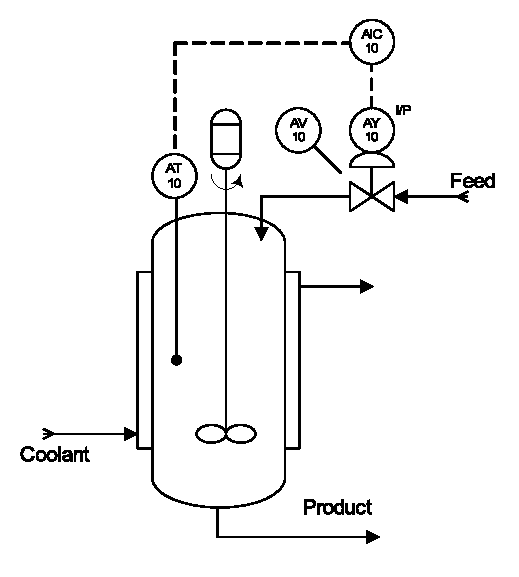
\includegraphics[width=0.5\linewidth]{Reactor02.eps}
\caption{Example 2 - CSTR System} \label{CSTR}
\end{figure}

Doing a mass balance, the system can be described by the following
model

\begin{align}
    \frac{dC_A(t)}{dt} & = \frac{F_r(t)}{V} \left[C_{Ai}-C_A(t)\right] - k_1 C_A(t) - k_3 C^2_A(t) \nonumber \\
    \frac{dC_B(t)}{dt} & = -\frac{F_r(t)}{V} C_B(t)+ k_1 C_A(t) - k_2 C_B(t)
    \label{system3}
\end{align}

\noindent where $F_r$ is the feed flow rate of product $A$, $V$ is
the reactor volume which is kept constant during the operation,
$C_A$ and $C_B$ are the reactant concentrations in the reactor,
and $k_i$ ($i=1,2,3$) are the reaction rate constants for the
three reactions.

In this case, the variables of interest are: the concentration of
$B$ in the reactor ($C_B$ as the controlled variable), the flow
through the reactor ($F_r$ as the manipulated variable), and the
concentration $C_{Ai}$ of $A$ in the feed flow (whose variation
can be considered as the disturbance). The kinetic parameters are
chosen to be $k_1 = 5/6 \ min^{-1}$, $k_2 = 5/3 \ min^{-1}$, and
$k_3 = 1/6 \ l \ mol^{-1} \ min^{-1}$. Also, is assumed that the
nominal concentration of $A$ in the feed ($C_{Ai}$) is $10 \ mol \
l^{-1}$ and the volume $V = 700 \ l$.

Using (\ref{system3}) and the parameters values, the
characterization of the steady-state for the process can be
obtained as it is shown in Fig.\ref{c_estatica}, for three
concentrations of $C_{Ai}$, where is easy to see the non-linearity
of the system.

\begin{figure}[htb!]
    \begin{center}
        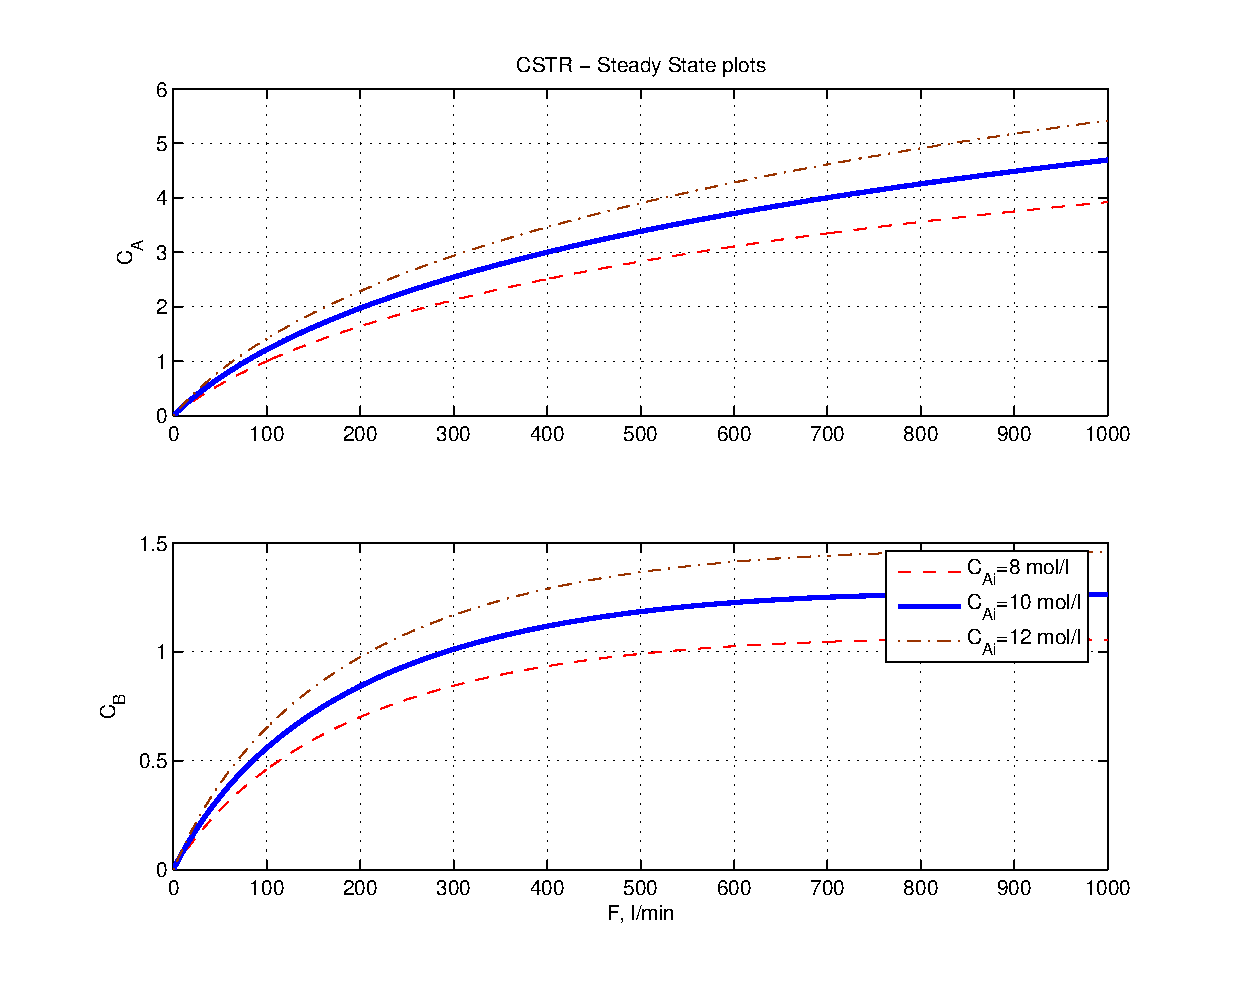
\includegraphics[width=0.7\linewidth]{c_estatica.eps}
        \caption{Example 2 - Steady-State characterization for the reactor}
        \label{c_estatica}
    \end{center}
\end{figure}

Initially, the system is at the steady-state (therefore the
operational point) with $C_{Ao} = 2.9175 \ mol \ l^{-1}$ and
$C_{Bo} = 1.10 \ mol \ l^{-1}$. From this, it can be selected the
measurement range for $C_B$ from $0$ to $1.5714 \ mol/l$ and the
capacity for the control valve with a maximum flow of $634.1719 \
l/min$ (variation range of the flow from $0$ to $634.1719 \
l/min$) \cite{arrietaETFA2008}. The signals ($y$, $u$, $r$) will
be in percentage ($0$ to $100\%$).

The sensor-transmitter element takes the form

\be
    y(t)_{\%} = \left(\frac{100}{1.5714}\right) C_B(t) \label{sensor}
\ee

\noindent and the control valve with a linear flow characteristic,

\be
    F_r(t) = \left(\frac{634.1719}{100}\right) u(t)_{\%} \label{actuator}
\ee

Fig.\ref{c_estatica2} shows the steady-state characterization,
taking into account elements represented by (\ref{sensor}) and
(\ref{actuator}). This is calling \emph{set
actuator-process-sensor} and from this is clearly that for the
selected steady-state, $r_o = 70 \%$ and $u_o = 60 \%$.

\begin{figure}[htb!]
    \begin{center}
        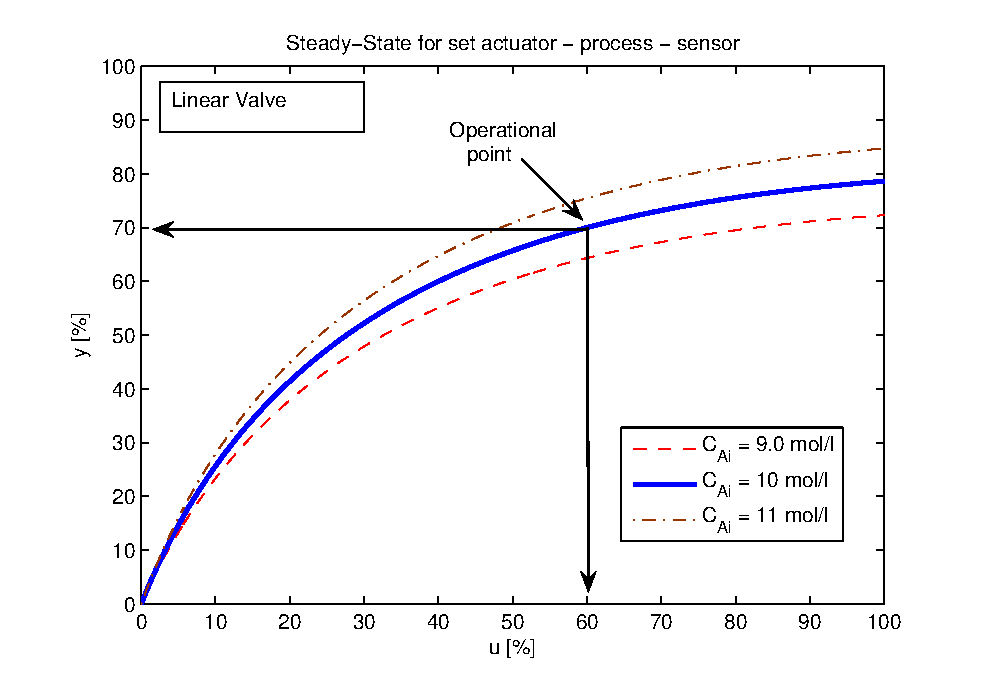
\includegraphics[width=0.7\linewidth]{c_estatica2.eps}
        \caption{Example 2 - Steady-State characterization for the set actuator-process-sensor}
        \label{c_estatica2}
    \end{center}
\end{figure}

It is assumed that changes in the set-point would be not bigger
than $10 \%$ and the possible disturbance in $C_{Ai}$, can variate
around $\pm 10 \%$. In Fig.\ref{process} can be seen the process
output (including the sensor and the control valve) and also the
FOPDT model for a step change in the process input ($y_u(t)$).

\begin{figure}[htb!]
    \begin{center}
        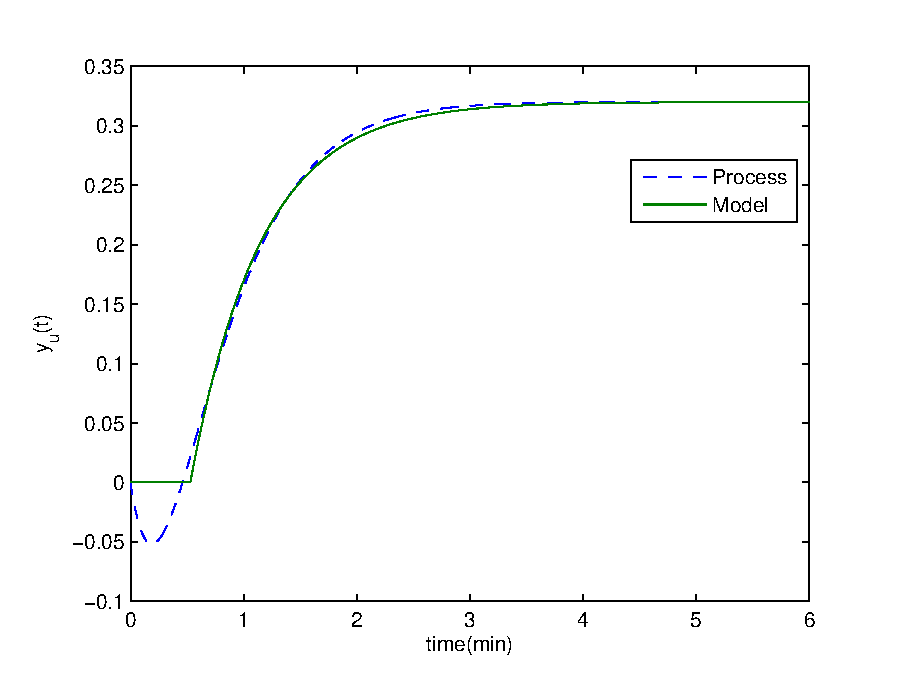
\includegraphics[width=0.7\linewidth]{FOPDT.eps}
       \caption{Example 2 - Reaction curve for process and FOPDT model} \label{process}
    \end{center}
\end{figure}

Using the identification method \cite{alfaro2006-1}, the
determined FOPDT model is

\be
    P_3(s) \approx \frac {0.3199 \me^{-0.5289 s}}{0.6238 s +1}
    \label{model_Pu}
\ee

From (\ref{model_Pu}), the application of the ISE tuning formulae
for optimal set-point and load-disturbance responses and also the
\emph{intermediate} $\overline{\gamma}_{\alpha}-autotuning$
provide the parameters for the PID controller that are shown in
Table \ref{PID_parameters3}.

\begin{table}[h!]
\begin{center}
\caption{Example 2 - PID Controller Parameters}
\begin{tabular}{c|ccc}
\hline \textbf{tuning}               &$K_p$ &$T_i$ &$T_d$\\ \hline
$set-point(sp)$                               &3.799  &0.707  &0.264 \\
$load-disturbance(ld)$                        &5.404  &0.494  &0.293 \\
\hline
$\overline{\gamma}_{\alpha=0.25}-autotuning$  &4.190  &0.609  &0.269 \\
$\overline{\gamma}_{\alpha=0.50}-autotuning$  &4.570  &0.577  &0.270 \\
$\overline{\gamma}_{\alpha=0.75}-autotuning$  &4.820  &0.551  &0.273 \\
\hline
\end{tabular}
\label{PID_parameters3}
\end{center}
\end{table}

Process outputs of the closed-loop system are shown in Fig.
\ref{y31}, first for a set-point step change of -10\%, follows by
a disturbance of +10\% and finally a new change in the set-point
of +5\%, all these situations using the three tuning modes
(set-point, load-disturbance and
$\overline{\gamma}_{\alpha}-autotuning$). Also, the control signal
($u(t)$) can be seen. It appears that, as expected, the control
signal is smoother for lower values of $\alpha$.

\begin{figure}[htb!]
    \begin{center}
        \includegraphics[width=0.7\linewidth]{y3outp1.eps}
       \caption{Example 2 - Process output for the non-linear control system operating in both servo and regulation modes} \label{y31}
    \end{center}
\end{figure}

A more comprehensive picture of the set-point change is shown in
Fig. \ref{y32}. In this case, it can be seen that, as expected,
the set-point tuning gives the better performance for servo
operation mode. Furthermore, the
$\overline{\gamma}_{\alpha}-autotuning$ provides a lower
degradation, respect to the optimal, than the load-disturbance
tuning.

\begin{figure}[htb!]
    \begin{center}
        \includegraphics[width=0.7\linewidth]{y3outp2.eps}
       \caption{Example 2 - Process output for the non-linear control system operating as servo} \label{y32}
    \end{center}
\end{figure}

The detail of load-disturbance attenuation is in Fig. \ref{y33}.
Similarly to the previous case, the load-disturbance tuning is the
one that gives better performance for regulation operation and the
performance degradation of the set-point tuning is greater than
the three cases for $\overline{\gamma}_{\alpha}-autotuning$.

\begin{figure}[htb!]
    \begin{center}
        \includegraphics[width=0.7\linewidth]{y3outp3.eps}
       \caption{Example 2 - Process output for the non-linear control system operating as regulator} \label{y33}
    \end{center}
\end{figure}

In general terms, it can be confirmed that the
$\overline{\gamma}_{\alpha}-autotuning$ gives a better performance
when the system operates in both servo and regulation modes. Also,
the control signal for the \emph{intermediate} tuning seems to be
\emph{smoother} than that provided by the optimal regulation
settings.

Table \ref{values_PDex3} shows the $\mathit{PD}$ and
$\mathit{WPD}$ indices and the improvement that can be achieve for
each case of the $\overline{\gamma}_{\alpha}-autotuning$.\\

\begin{table}[htb!]
\begin{center}
\caption{Example 2 - $\mathit{PD}$ and $\mathit{WPD}$ values for
the non-linear CSTR system and the improvement obtained with
$\overline{\gamma}_{\alpha}-autotuning$}
\begin{tabular}{c|cc|ccc}
\hline \textbf{tuning}       &$PD_{sp}$  &$PD_{ld}$ &$WPD_{\alpha=0.25}$ &$WPD_{\alpha=0.50}$ &$WPD_{\alpha=0.75}$\\
\hline
$set-point(sp)$                               &-          &0.3284 &0.0821 &0.1642 &0.2463\\
$load-disturbance(ld)$                        &0.5316     &-      &0.3987 &0.2658 &0.1329\\
$\overline{\gamma}_{\alpha=0.25}-autotuning$  &0.0192     &0.1398 &0.0493 &- &-\\
$\overline{\gamma}_{\alpha=0.50}-autotuning$  &0.0706     &0.0470 &- &0.0588 &-\\
$\overline{\gamma}_{\alpha=0.75}-autotuning$  &0.1334     &0.0038 &- &- &0.0362\\
\hline \hline
improvement in \% of                          &            &            & & &\\
\hline
$\overline{\gamma}_{\alpha=0.25}-autotuning$  &96.39\%(ld) &57.73\%(sp) &39.95\%(sp) &- &-\\
                                              &            &            &87.63\%(ld) &- &-\\
$\overline{\gamma}_{\alpha=0.50}-autotuning$  &86.72\%(ld) &85.99\%(sp) &- &64.19\%(sp) &-\\
                                              &            &            &- &77.88\%(ld) &-\\
$\overline{\gamma}_{\alpha=0.75}-autotuning$  &74.91\%(ld) &99.15\%(sp) &- &- &85.30\%(sp)\\
                                              &            &            &- &- &72.76\%(ld)\\
(respect to)                                  &            &            & & &\\
\hline
\end{tabular}
\label{values_PDex3}
\end{center}
\end{table}

%-----------------------------------------
%
\section{Conclusions}
\label{conclusions}
%
%-------------------------------------------

In process control it is very usual to have changes in the
set-point, as well as in the disturbance. This causes the need to
face with both servo and regulatory control problems. For 1-DoF
PID controllers, when the tuning objective is different to the
real system operation, a degradation in the performance is
expected and it can be evaluated. A reduction in the overall
Performance Degradation can be obtained by searching an
\emph{intermediate} controller between the optimal ones proposed
for set-point and load-disturbance tunings.

Autotuning formulae have been presented with the aim to minimize
the Weighted Performance Degradation, expressed as a combination
depending of the balance between the total time that the system
operates in servo and regulation modes. This is the main
contribution of this paper because it is a novel feature that
allows to select the tuning according to a general qualitative
specification of the control system operation.

Results are given for PID controllers, in order to get results
closer to industrial applications. The examples have shown the
improvement obtained with each one of the
$\overline{\gamma}_{\alpha}-autotuning$ cases.

Even if the results were presented and exemplified using the ISE
performance criteria, it could be possible to reproduce a similar
methodology to other PID controllers, like the one that uses
derivative action is applied just to process output, or to other
PID tunings with different performance objectives.

%-------------------------------------------
%
\section*{Acknowledgments}
%
%-------------------------------------------

This work has been supported by: the Spanish CICYT program under
grant DPI2007-63356, the University of Costa Rica and the MICIT
and CONICIT of the Government of the Republic of Costa Rica.

Also, the financial support given by the AGAUR research funds
BE-DGR 2008, enabled O. Arrieta to perform a research period at
the Dipartimento di Elettronica per l'Automazione of the
University of Brescia, Italy.


\vspace{1cm}

\bibliographystyle{elsarticle-num}
\bibliography{GammaS}

\end{document}
